\section{Entanglement in front of a thermal shield}\label{sec:5:thermal-entanglement}
The entanglement generation between the two particles depends heavily on the variation of the separation between the shield and the particles, as has been seen in \cref{cha:entanglement-generation}.
The vibrating shield can be interpreted as varying the separation and angle of the cat-state in front of the plate - visualized in \cref{fig:5:vibrating-translation-to-variations}.
\begin{figure}[!htbp]
  \centering
  \def\svgwidth{\textwidth}
  \input{./../figures/plate-vibration.pdf_tex}
  \caption{For a large $r_s \gg R$ and locally flat shield, the thermal vibrations with amplitude $z$ can be interpreted as a static shield where the particle $A$ (shown in the figure) is placed at $L+\Delta L$ at angle $\theta$ and particle $B$ is places at $L-\Delta L$ with angle $-\theta$ where both variations depend on the amplitude. At low vibrational frequencies $1/\omega \approx t_\mathrm{max}$ the amplitude can be assumed to be static during a experimental run and for each measurement thermally distributed around $\mean{z}=0$ with $\Delta z$ given by eq. \eqref{eq:5:amplitude-variance}.}
  \label{fig:5:vibrating-translation-to-variations}
\end{figure}
This is only a good approximation for shields larger than the particles radius $r_s \gg R$ and low vibrating frequencies $1/\omega \approx t_\mathrm{max}$ and can therefore be used well to describe the highly disturbing first few modes on a large shield.
Furthermore, this interpretation is possible because as shown in \cref{sec:3:imperfect-plates}, the Casimir interaction between a sphere and a tilted plane does not differ from the interaction between a flat plane.
Contrary to the problem considered in \cref{cha:entanglement-generation}, here only the thermal amplitude $z_{kl}$ is a independent random variable distributed around $\mean{z_{kl}} = 0$ with standard deviation $\Delta z_{kl}$ given by eq. \eqref{eq:5:amplitude-variance}. 
Both, the variations in the particle-shield separation $\Delta L$ as well as in the angle $\theta$ are correlated to the amplitude $z$.
For a large shield, this can be understood as
\begin{equation}
  \theta = \arctan(z \abs{\nabla u}) \approx z \abs{\nabla u} \quad \text{and} \quad \Delta L = z \abs{u}
\end{equation}
where $\nabla u$ is the gradient of the shape of the vibrational mode.
Performing similar calculations as done before in \cref{cha:entanglement-generation}, the averaged density matrix $\mean{\rho}$ dependent on $\Delta z_{kl}$ can be calculated.
The entanglement quantified by the logarithmic negativity \cite{Plenio_2005} introduced in \cref{sec:2:entanglement-measures} dependent on the temperature $T$ is shown in \cref{fig:5:entanglement-temperature}.
\begin{figure}[!htbp]
  \centering
  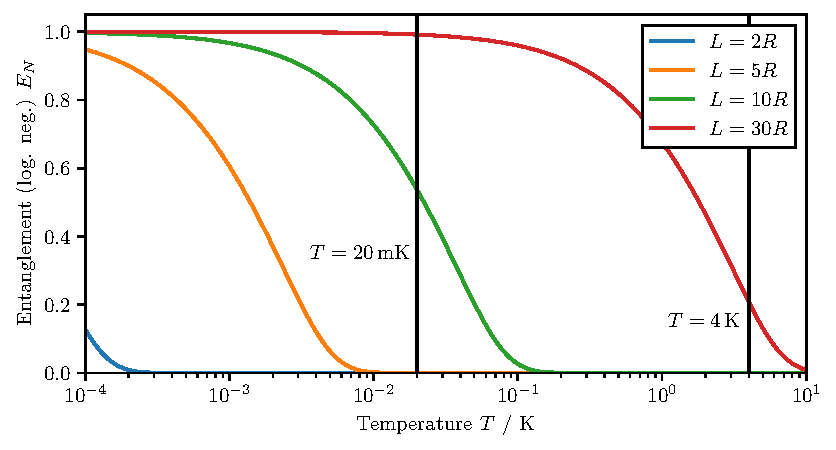
\includegraphics[width=\textwidth]{./../figures/vibrations/entanglement-shield-T-L.pdf}
  \caption{Entanglement between the particles (parallel orientation) in front of a thermal shield in the first mode $(1,0)$ at temperature $T$ for different particle-shield separations $L$.}
  \label{fig:5:entanglement-temperature}
\end{figure}
This is not surprising considering that the thermal amplitudes $\Delta z_{1,0} \approx 9 \times 10^{-11}\si{m}$ at $20\si{mK}$ which is comparable with the previously calculated values for $\Delta L_\mathrm{crit}$ in \cref{cha:entanglement-generation}.
Surprisingly this result does not change for different shield radii - at least as long as the condition $r_s \ll R$ is fulfilled and the shield shape can locally be linearized.
This is because the gradient $\abs{\nabla u} \propto 1/r_s$ which perfectly cancels with the dependence on $z \propto r_s$ leaving $\theta$ independent of $r_s$. 
If the cat-state orientation is now chosen parallel to the shield, the dependence on $\Delta L$ is irrelevant leaving the final resulting entanglement independent of $r_s$. 



\subsection{Analytic dynamics}
Surprisingly the influence of the thermal shield on entanglement generation can be calculated analytically.
\begin{align}\label{eq:5:hamiltonian}
\begin{split}
  \op{H} = \sum_{\substack{m\in\{(k,l)\}\\ k \geq 1,\ l \geq 0}} & \hbar \omega_m \left(\op{a}^\dagger_m \op{a}_m + \frac{1}{2}\right) \\
  &+ \left[g^{1,1}_\mathrm{Grav} + \left(g^1_\mathrm{A,m,Cas} +
  g^1_\mathrm{B,m,Cas}\right)(\op{a}_m + \op{a}^\dagger_m)\right] \ketbra{\psi^1_A \psi^1_B} \\
  &+ \left[g^{1,2}_\mathrm{Grav} + \left(g^1_\mathrm{A,m,Cas} + g^2_\mathrm{B,m,Cas}\right)(\op{a}_m + \op{a}^\dagger_m)\right]\ketbra{\psi^1_A \psi^2_B} \\
  &+ \left[g^{2,1}_\mathrm{Grav} + \left(g^2_\mathrm{A,m,Cas} + g^1_\mathrm{B,m,Cas}\right)(\op{a}_m + \op{a}^\dagger_m)\right]\ketbra{\psi^2_A \psi^1_B} \\
  &+ \left[g^{2,2}_\mathrm{Grav} + \left(g^2_\mathrm{A,m,Cas} + g^2_\mathrm{B,m,Cas}\right)(\op{a}_m + \op{a}^\dagger_m)\right]\ketbra{\psi^2_A \psi^2_B}
\end{split}
\end{align}
where $g^{ij}_\mathrm{Grav}$ is the gravitational coupling between the states $\ket{\psi^i_A}$ and $\ket{\psi^j_B}$.
The Casimir interaction between state $\ket{\psi_{A(B)}^i}$ and the shield is denoted by $\tilde{g}^i_\mathrm{A(B),\,m,\,Cas}$. These couplings are dependent on the amplitude $\op{z}_{m} = \sqrt{\hbar/2\tilde{m}\omega_m} (\op{a}_m + \op{a}^\dagger_m)$ and the shape $u_{m}(r_{A(B)})$ of the vibrational mode $m=\{(k,l)\}$ at the position $r_{A(B),i}$ of the cat state:
\begin{equation}
  \tilde{g}^i_\mathrm{A(B),\,m,\,Cas} = \frac{\hbar c \pi^3}{720} \left(\frac{\varepsilon_r - 1}{\varepsilon_r + 1}\right)\varphi(\varepsilon_r) \frac{R}{(\mathscr{L} + \op{z}_m u_m(r))^2} \approx g_\mathrm{PFA} \left(\frac{1}{\mathscr{L}^2} + \frac{2 \op{z}_m u_m(r_{A(B),i})}{\mathscr{L}^3}\right) .
\end{equation}
Ignoring the first term in the expansion, which just produces a global phase in the evolved system, the couplings $g_\mathrm{Cas}$ appearing in eq. \eqref{eq:5:hamiltonian} are finally given by
\begin{equation}
  g^i_\mathrm{A(B),\,m,\,Cas} = g_\mathrm{PFA} \frac{2u_m(r_{A(B),i})}{\mathscr{L}^3} \sqrt{\frac{\hbar}{2 \tilde{m} \omega_m}} .
\end{equation}
It is possible to analytically calculate the time evolution of a system consisting of the initial state $\rho_\mathrm{system}$ (given by eq. \eqref{eq:2:initial-state}) combined with the infinite vibrational modes $\rho_\mathrm{th}$ of the thermal shield
\begin{equation}
  \rho_0 = \bigotimes_{m\in\{(k,l)\}} \left(\rho_\mathrm{th,\,m}\right) \otimes \rho_\mathrm{system} .
\end{equation}
These thermal states can be expanded into coherent states $\ket{\alpha} = \op{D}(\alpha)\ket{0}$ as \cite{Steiner_2024}
\begin{equation}
  \rho_\mathrm{th,m} = \frac{1}{Z} \sum_{n=1}^{\infty} e^{-\beta \hbar \omega_m (n + 1/2)} \ketbra{n} = \int \dd \alpha^2 \frac{1}{\pi \bar{n}} e^{-\frac{\abs{\alpha}^2}{\bar{n}}} \ketbra{\alpha}
\end{equation}
where $\bar{n}$ is the average occupation number. The time evolution of the particle-system $\rho_\mathrm{system}(t) = \tr_{th}\left\{\rho(t)\right\}$ can be calculated by tracing out all states corresponding to the thermal shield.

\begin{figure}[!htbp]
  \centering
  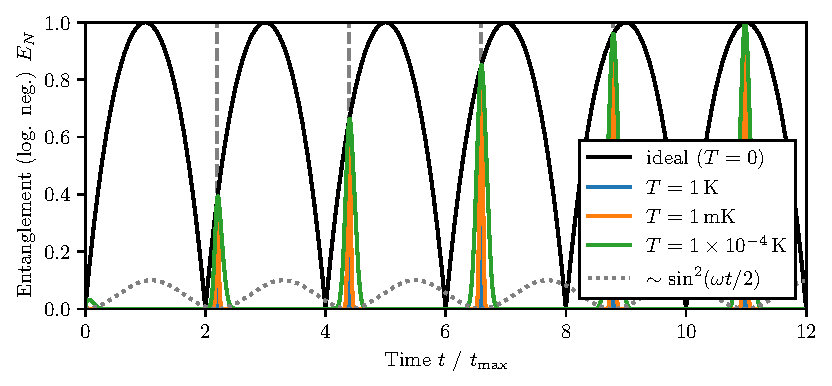
\includegraphics[width=\textwidth]{./../figures/vibrations/entanglement-hamiltonian.pdf}
  \caption{Entanglement dynamics in front of a thermal shield in mode $(1,0)$ at different temperatures. Only at specific times $2\pi k / \omega_{1,0},\ k\in\mathbb{N}$, entanglement is observable. This behavior is expected and aligns with the findings in Ref. \cite{Pedernales_2022}.}
\end{figure}

\begin{figure}[!htbp]
  \centering
  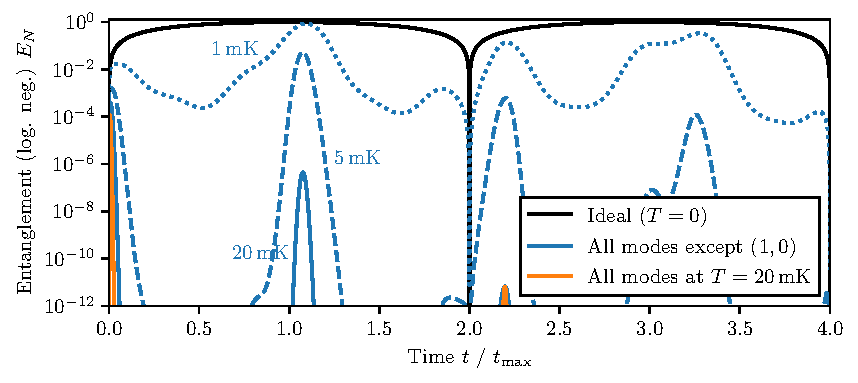
\includegraphics[width=\textwidth]{./../figures/vibrations/entanglement-multiple-modes.pdf}
  \caption{Entanglement dynamics in front of a thermal shield. In orange, the first 50 modes have been used in the numeric calculation. The effect of all remaining modes is around $1.7 \times 10^{-11}\,\%$. In blue, all modes except the first mode $(1,0)$ have been considered at different temperatures ranging vom $1\si{mK}$ up to $20\si{mK}$. The particle-shield separation is fixed at $L = 2R = 20\si{\mu m}$.}
\end{figure}

\begin{figure}[!htbp]
  \centering
  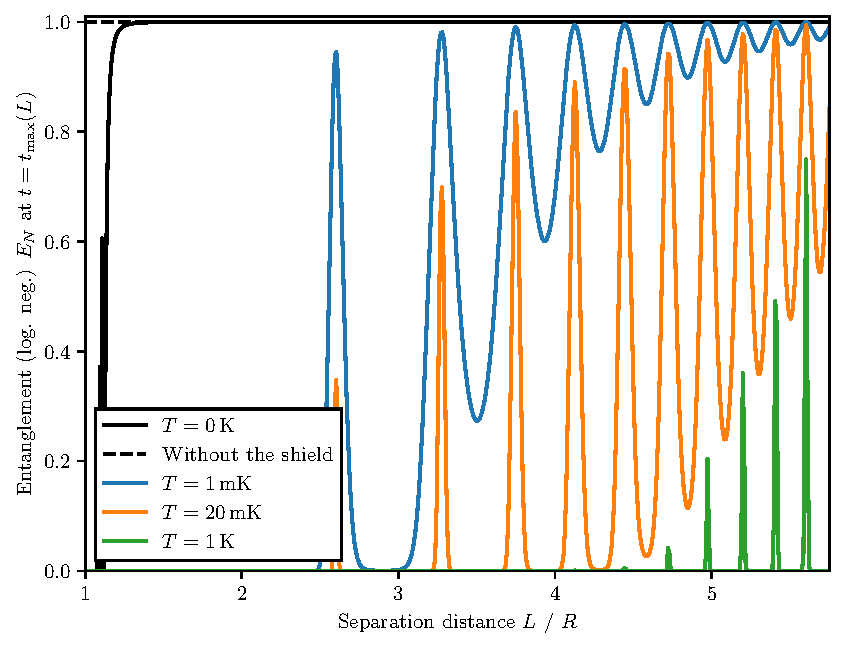
\includegraphics[width=\textwidth]{./../figures/vibrations/all-modes-maximum-entanglement-L-t-max.pdf}
  \caption{All modes, Entanglement at t-max}
\end{figure}


\subsection{Small shields}
